\documentclass[a4paper,10pt,openany,oneside]{report}

\usepackage{amsfonts}
\usepackage{amsmath}
\usepackage{amssymb}
\usepackage[french]{babel}
\usepackage{changepage}
\usepackage{color}
\usepackage{enumitem}
\usepackage{fancyhdr}
\usepackage[T1]{fontenc}
\usepackage[left=3cm,right=3cm,top=3cm,bottom=3cm,headsep=1cm]{geometry}
\usepackage{graphicx}
\usepackage[hidelinks]{hyperref}
\usepackage[utf8]{inputenc}
\usepackage{listings} %Pour le code
\usepackage{titlepic}
\usepackage{wrapfig}

\setitemize{topsep=5pt}
\setlength{\parindent}{1em}

\definecolor{dkgreen}{rgb}{0,0.6,0}
\definecolor{gray}{rgb}{0.5,0.5,0.5}
\definecolor{mauve}{rgb}{0.58,0,0.82}
\definecolor{myblue}{rgb}{0,0,1}
\definecolor{bonus}{rgb}{1,0.7,0}

\newcommand\blfootnote[1]{%
  \begingroup
  \renewcommand\thefootnote{}\footnote{#1}%
  \addtocounter{footnote}{-1}%
  \endgroup
}

\lstset{frame=tb,
  language=C++,
  aboveskip=3mm,
  belowskip=3mm,
  showstringspaces=false,
  columns=flexible,
  basicstyle={\small\ttfamily},
  numbers=left,
  numberstyle=\normalsize,
  numbersep=7pt,
  numberstyle=\tiny\color{gray},
  keywordstyle=\color{blue},
  commentstyle=\color{dkgreen},
  stringstyle=\color{mauve},
  breaklines=true,
  breakatwhitespace=true,
  tabsize=4
}

\begin{document}
\begin{titlepage}
\titlepic{
\includegraphics[scale=0.2]{img/iconCB.png}}
\title{City Builder}
\author{Damian Petroff, Sergiy Goloviatinski, Raphaël Margueron}
\date{\today}
\maketitle
\end{titlepage}

%------
\thispagestyle{empty}
\pagebreak
\thispagestyle{empty}
%------
\chapter*{Abstract}
\thispagestyle{empty}
Abstract content
\pagebreak
%------
\thispagestyle{empty}
\tableofcontents
\thispagestyle{empty}
%------
\chapter*{Introduction}
\setcounter{page}{1}
\paragraph{}
L'industrie vidéo-ludique est aujourd'hui un marché grandissant de manière notoire et notre intérêt pour les diverses facettes que ce domaine propose a inévitablement influencé notre choix.
En effet, la conception d'un jeu-vidéo n'est de loin pas une mince affaire. Dans ce rapport nous allons présenter comment nous avons relevé le défi et notre approche sur sa conception et sa réalisation.

Il est nécessaire de prendre note qu'aucun de nous trois n'avait réalisé ni même conceptualisé de jeu-vidéo auparavant, malgré cela, c'est un domaine très intéressant et très complet qui laisse part à la créativité autant sur le plan artistique que scientifique du fait de la diversité des corps de métier nécessaires à l'élaboration d'un tel produit. Le dessin, la sculpture, l'architecture, la musique, la littérature et le cinéma sont quelques uns des arts présents dans la conception d'un jeu-vidéo et nous sommes trois développeurs possédant peu de connaissances en création de contenu audiovisuel, il est donc évident que nous nous sommes orienté vers un jeu de type réflexion ou gestion, qui contient relativement beaucoup d'algorithmie. Le but n'étant pas non plus de créer un sudoku.

\paragraph{Vers un city builder :}
L'idée d'un jeu portant sur la conception et la gestion d'une ville nous a paru appropriée, chacun de nous connait un tant soit peu le sujet, ayant joué à des grosses licences comme "\textit{Cities: Skylines}" de Colossal Order\footnote{Colossal Order : \textcolor{blue}{\url{www.colossalorder.com}}}
\blfootnote{\hspace{7pt}Figure 1. Source de l'image : \href{https://www.reddit.com/r/CitiesSkylines/comments/3mubt5/finally_my_first_city_in_more_then_80_hours_i/}{\texttt{\textcolor{blue}{www.reddit.com/r/CitiesSkylines}}}}
 ou encore "\textit{SimCity}" de Electronics Arts\footnote{Electronics Arts : \textcolor{blue}{\url{www.ea.com}}} pour ne citer qu'elles. Ce type de jeu de gestion laisse place à une certaine liberté de contenu (comme les bâtiments disponibles, les ressources nécessaires, etc.). Nous avons donc pris la décision de créer un produit de la même nature, en version extrêmement plus modeste évidement.
\begin{center}
	\begin{figure}[h]
	\centering
	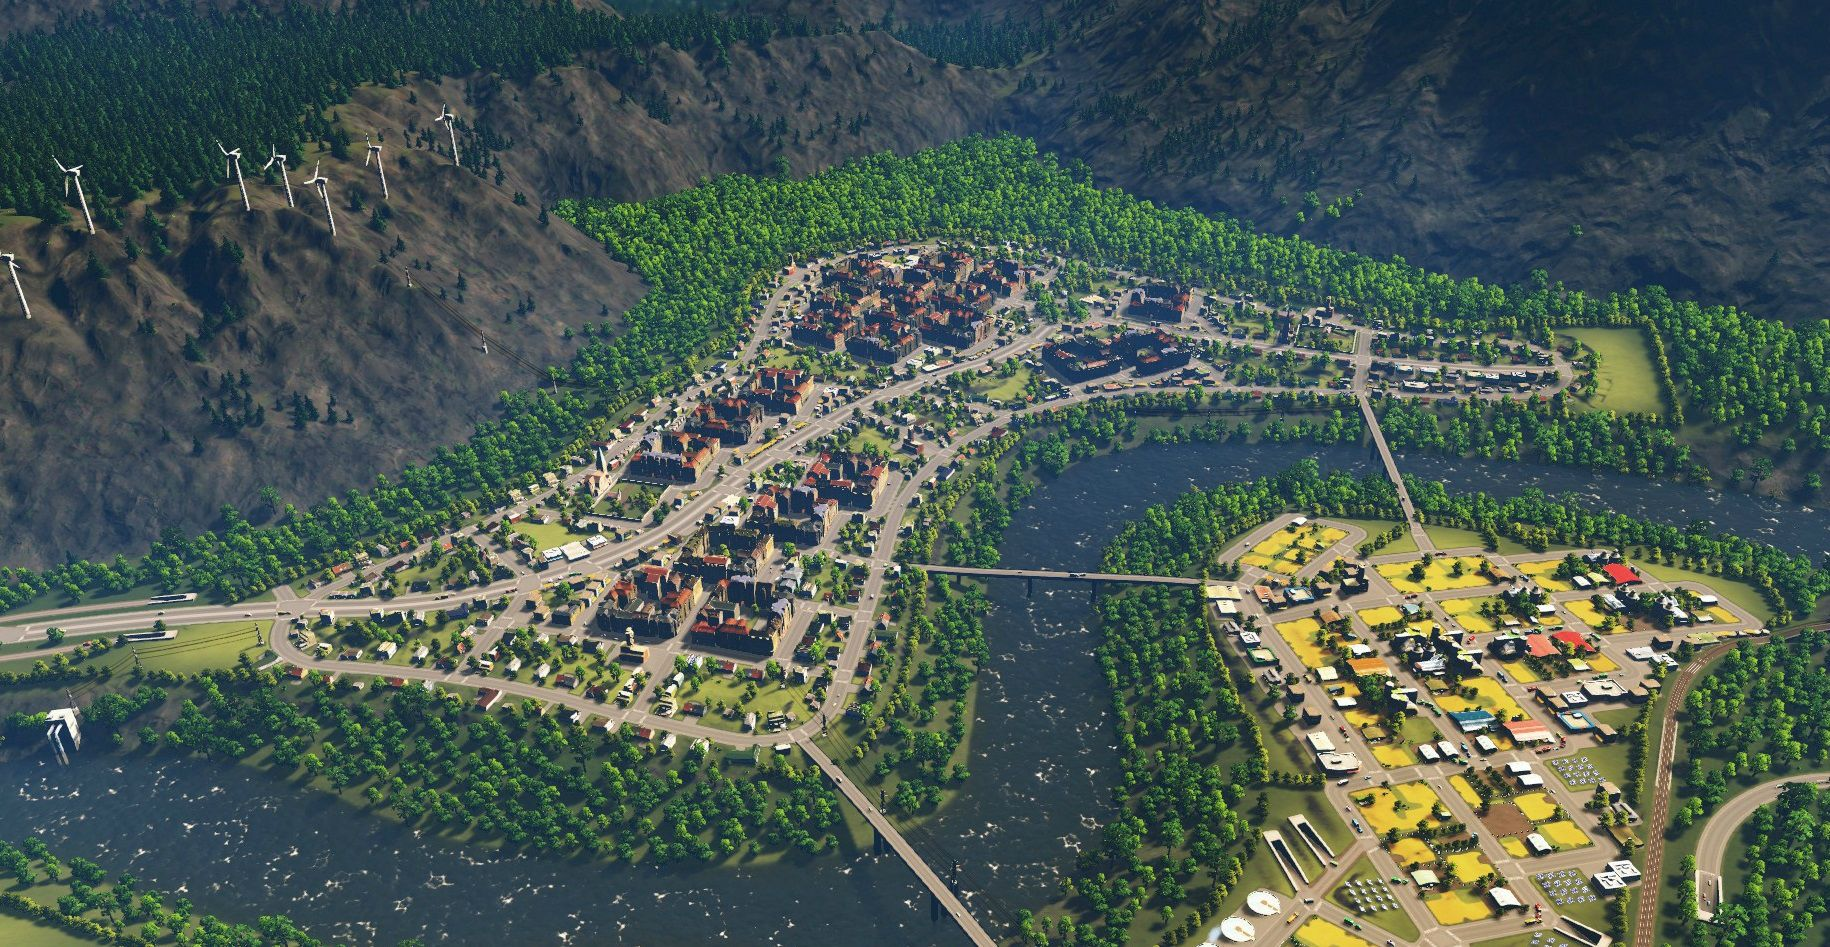
\includegraphics[width=0.9\textwidth]{img/img_intro_cscity.jpg}
	\caption{\label{fig:Cities: Skylines city}Un village sur Cities : Skylines}
	\end{figure}
\end{center}

\thispagestyle{empty}
\paragraph{}
Le but principal du projet est de produire un city builder avec des interactions basiques, un certain panel d'actions possibles rendant le jeu "jouable" et significativement unique. L'application doit être stable et répondre aux spécifications (cf. section 1.1 Spécifications). Le joueur a la possibilités de commencer une nouvelle partie avec des paramètres personnalisés et de reprendre une partie déjà commencée (principe de sauvegarde). L'application doit être codée en C++ via le framework Qt qui permet de faciliter l'affichage et la gestion des éléments graphiques et des conteneurs. Les éléments du framework Qt appris au cours aident à concevoir les composants graphiques principaux nécessaires.
\paragraph{}
Ce rapport décrit les étapes de réflexion, conceptualisation et réalisation des différentes facettes du projet. En premier lieu, nous analyserons les besoins du projet et ses spécifications. Ensuite nous détaillerons sa conception, notre planification et notre stratégie de développement. À la suite de quoi nous expliquerons la phase de développement en détail. Enfin, nous proposerons un bilan du projet suivi d'une conclusion traitant de notre ressenti par rapport à cette expérience.

\chapter{Analyse des besoins}
\thispagestyle{headings}
\section{Exigences fonctionnelles}
\subsection{Spécifications}
Voici les spécifications principales\footnote{Par spécifications principales, on entend les fonctionnalités nécessaires, sans citer celles bonus, qui viendront à la section suivante} du projet :
\subsubsection{Général}
\begin{itemize}
\item Possibilité de créer une nouvelle partie avec des paramètres personnalisés comme :
\begin{itemize}
\item La taille de la carte;
\item La graine de génération aléatoire;
\item La difficulté;
\item Le nom de la partie.
\end{itemize}
\item Possibilité de charger une sauvegarde d'une partie
\item Possibilité de générer une carte aléatoire
\item Le jeu est en plein écran
\item Utilisation de contenu audio (musique d'ambiance, événements)
\item Possibilité de voir toute la carte à la fois ou alors de zoomer puis de se déplacer en haut, en bas, à gauche et à droite
\item La carte est divisée en cases carrées, certains bâtiments peuvent utiliser plusieurs cases
\end{itemize}
\subsubsection{Mécaniques de gameplay}
L'application doit permettre de :
\begin{itemize}
\item construire des routes;
\item construire des habitations;
\item construire des bâtiments publiques qui ont un effet sur la population;
\item voir le rayon d'effet d'un tel bâtiment lors de sa construction;
\item détruire des éléments déjà construits;
\item construire un élément qu'à condition d'en avoir les moyens financiers;
\item construire un élément qu'à condition d'avoir déjà construits le ou les éléments requis à sa construction (exemple : Construire une tour Eiffel ne peut se faire que dans un ville relativement grande.)
\item créer une économie via des coûts de certaines infrastructures;
\item gérer les frais imposés aux habitants ;
\item 
\end{itemize}

\subsubsection{Interface utilisateur}
Le HUD\footnote{\textit{Head Up Display} : Communication graphique des informations avec le joueur} du jeu comporte :
\begin{itemize}
\item Un espace d'affichage des données de jeu comme la fortune, la population, le bonheur, le nom de la partie, etc.;
\item Un menu d'options, sauvegarde, quitter la partie, etc.;
\item Le carte en elle-même;
\item Un onglet de construction de bâtiments;
\end{itemize}

\subsubsection{Rendu graphique}
\begin{itemize}
\item Le jeu est en 2.5D (2D isométrique)
\item Une différence visuel entre terrain constructible et non-constructible
\item Une différence visuelle entre les différents types de bâtiments, via des couleurs par exemple.
\end{itemize}

\subsubsection{Bâtiments}
Le panel de bâtiments doit être relativement complet et toucher à plusieurs domaines comme :
\begin{itemize}
\item \textbf{La santé : }linique, hôpital, cimetière, crématoire, sauna, laboratoire médicaux, dépôt pour hélicoptère médical, etc.
\item \textbf{Les services d'urgence : }caserne de pompier, dépôt pour hélicoptère de pompier / Canadair, tour de garde, unité de réponse en case de catastrophe, bunker, antenne radio, etc.
\item \textbf{L'éducation : }école primaire, école secondaire, école professionnelle, lycée, université, faculté, etc.
\item \textbf{Les transports : }dépôt de bus, station de bus, arrêt de bus, pareil pour tram, métro, taxi, train, bateau, avion, etc.
\item \textbf{Les loisirs : }restaurant, centre commercial, bibliothèque, parc, place de jeu, jardin botanique, parc d'attraction, terrain de sport, lieu de pêche, étable, skate park, etc.
\item \textbf{Les monuments : }stade de foot, Tour Eiffel, statues, mémoriaux, fontaines, etc.
\end{itemize}


\subsection{Spécifications \textcolor{bonus}{bonus}}
Cette section tient d'indication sur quelques idées que nous avions au cas où le temps nous le permettrait.

\subsubsection{Général}
\begin{itemize}
\item
\end{itemize}

\subsubsection{Mécaniques de gameplay}
\begin{itemize}
\item Impossible de construire un bâtiment sans route qui le borde
\item Filtre pour afficher la quantité de bonheur apportée par case (somme des effets de tous les bâtiments). Permet de savoir quelles sont la zone la plus ou moins heureuse de la ville.
\item Système de quêtes pouvant servir de tutoriel, par exemple:
\begin{itemize}
\item Construire une route
\item Construire quatre maisons
\item Récompense : 200 \$ et déblocage d'un bâtiment
\end{itemize}
\item Gérer plusieurs difficultés
\end{itemize}

\subsubsection{Interface graphique}
\begin{itemize}

\item Une minimap affichable ou non sur laquelle il serait possible de cliquer pour se rendre au bon endroit directement
\end{itemize}

\subsubsection{Rendu graphique}
\begin{itemize}
\item Nos propres textures de bâtiments et de routes grâce auxquelles il serait possible de créer un thème comme le futurisme, le western ou même une ville technologiquement évolutive dans le temps
\item Textures adaptatives des routes, gestion des virages et des croisées
\item Temps de construction d'un bâtiment, sous forme d'un chantier animé
\end{itemize}



\section{Exigences non-fonctionnelles}
\subsection{Codage}
\subsection{Portabilité}
\subsection{Ergonomie}
\subsection{Efficience}
\subsubsection{Temps de réponse}
\subsubsection{Utilité des ressources}
\subsection{Maintenabilité}
\section{Cas d'utilisation}


\chapter{Conception}
\thispagestyle{headings}
\section{Stratégie de conception}
\subsection{Planification initiale}

\section{Architecture logicielle}
\subsection{Schéma procédural}
\subsection{Diagramme de classe}
\subsection{Convention de codage}

\section{Interface utilisateur}
Cette section traite des choix faits sur les possibilités d'interactions de l'utilisateur avec l'application. En premier lieu sera présenté le launcher, puis le client. 
\subsection{Launcher}
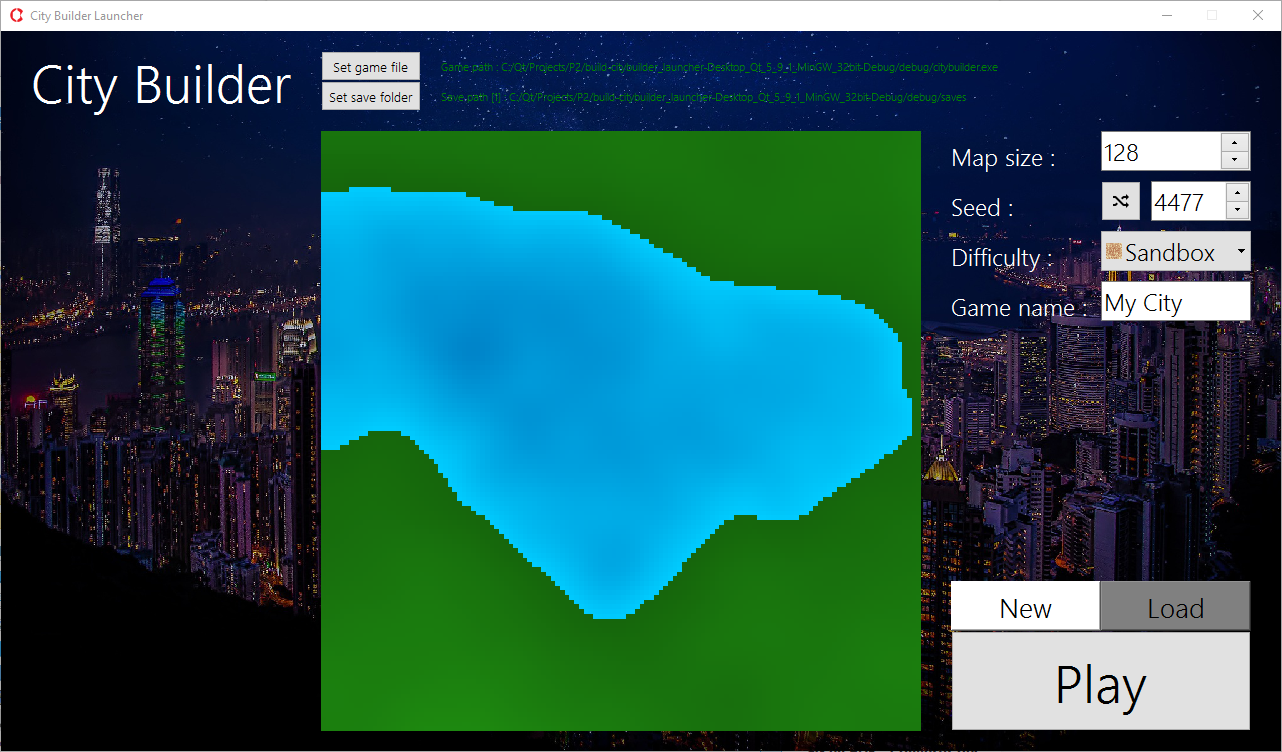
\includegraphics[width=\textwidth]{img/ui_launcher.png}
\subsubsection{Interactions et raccourcis}
\subsubsection{Esthétique}
\subsection{Client}
$Insérer une image$
\paragraph{}
L'interface graphique se divise en 3 parties:\\\\
$TopView$ : Vue fixe se trouvant toujours en haut de l'interface et qui contient:
\begin{itemize}
\item L'heure et la date dans le jeu
\item Des indicateurs d'argent, de bonheur et de population disponible pour le joueur avec le delta entre chaque seconde
\item Une $SpinBox$ permettant de régler le niveau d'impôts
\item Le nom de la carte, pouvant être modifié si on clique dessus
\item Des $Slider$ pour régler le volume de la musique et des effets
\item Des boutons pour charger,sauvegarder et quitter la partie
\item La valeur de la seed utilisée pour générer la carte
\end{itemize}
$MapView$ : Contient le terrain de jeu, les différents raccourcis claviers (même quand cette vue n'a pas le focus) et actions de souris qui sont dans son focus influencent sur cette vue:
\begin{itemize}
\item Translation dans la vue (Raccourcis: A S D W ou flèches directionnelles)
\item Zoom dans la vue (Raccourcis : + - ou molette de la souris)
\item Afficher/masquer la grille (Raccourci: G)
\item Afficher/masquer les rayons d'effets de tous les bâtiments qui en ont un (Raccourci: F)
\item Afficher le rayon d'effet d'un bâtiment s'il en a un quand un clique dessus
\end{itemize}
$GuiView$ : Vue contenant les boutons permettant de:
\begin{itemize}
\item Choisir la catégorie de bâtiment à poser (Raccourcis clavier disponible depuis n'importe quelle vue: F1 à F9)
\item Les différents bâtiments à poser selon la catégorie choisie (Raccourcis claviers de 1 à 0)
\item Un bouton pour poser des routes disponibles dans toutes les catégories (Raccourci: Q)
\item Un bouton pour supprimer un bâtiment/route disponible dans toutes les catégories (Raccourci: R)
\end{itemize}
\subsubsection{Interactions et raccourcis}

\subsubsection{Esthétique}


\chapter{Développement et réalisation}
\thispagestyle{headings}
\section{Fonctionnalités du launcher}
\subsection{Création d'une partie}
\subsection{Chargement d'une partie}
\section{Fonctionnalités du client}
\subsection{Génération des sols}
Pour la gestion du terrain, nous avons décidé d'avoir deux types de sol : l'eau et l'herbe. Sur l'herbe, il est possible d'ajouter des bâtiments et sur l'eau non.

Pour pouvoir avoir des cartes auto-générée, nous avons décide d'utiliser un algorithme de bruit de Perlin. Nous n'allons pas aller dans les détails du fonctionnement du bruit de Perlin, dans ce rapport. Mais son principe est le suivant: il permet d'avoir des nombres aléatoires qui sont proche les uns de autres en function d'une seed(pour l'aléatoire, initialisé au début) et de 1, 2 ou X dimensions (trois dans celui que nous avons utilisés, mais que 2 utilisés). Vu que les outputs de la function de bruit de Perlin sont les mêmes quand nous utilisons les mêmes inputs. Nous pouvons la considérer comme une fonction à plusieurs variables (qui sont les dimensions et la seed). Changer la seed donne des résultats complètement différent mais changer les autres variables change peu entre chaque valeur.

\[bruit = perlin(seed, x, y, z)\]

Les nombres aléatoires que nous récupérons de la function sont des nombres flottant entre 0 et 1.
Leurs distribution sont sous la forme d'une distribution normal.
\[y=e^{-x^{2}}\]

Pour pouvoir générer la carte nous parcourons toutes les cases de la carte (selon x et y). Et "nous déplaçons sur le fonction de Perlin" d'un certain offset (qui est un multiple des index des cases).
\subsection{Gestion des cases de la carte}
Nous stockons les cases de la carte dans un $QArray$ d'une longueur $nbCases^{2}$

Une case à la coordonnée $X;Y$ dans la grille de cases représentant la carte correspond à l'élément se trouvant à l'indice $X+Y nbCases$ dans le $QArray$

Une case de la carte est représenté par la classe $MapTile$ dérivé de la classe $QGraphicsRectItem$ et contient les attributs suivants:
\begin{itemize}
\item bOccupied (boolean): dit si la case est occupée par un bâtiment ou de l'eau ou pas
\item x (int): coordonnée en x dans la matrice contenant les MapTile
\item y (int): coordonnée en y dans la matrice contenant les MapTile
\item bId (int): id du type de bâtiment (tous les hôpitaux ont la même bId p. ex)
\item unique BId (int): id unique du bâtiment (chaque bâtiment posé aura une id unique différente)
\item mainTileX (int): coordonnée en X de la case principale (en haut à gauche), utile pour les bâtiments d'une largeur ou hauteur supérieures à 1
\item mainTileY (int): même chose que mainTileX mais la coordonnée Y
\item buildingWIdth (int): largeur en nombre de cases d'un bâtiment
\item buildingHeight (int): hauteur en nombre de cases d'un bâtiment
\item bPix (boolean): indique si la case a une texture ou pas
\item buildImage ($QGraphicsPixmapItem*$): Pointeur vers la texture du bâtiment/route qui se trouve sur la case
\end{itemize}
\subsection{Routes et bâtiments}
Pour la gestion des routes et des bâtiments nous sommes parti sur une approche plutôt simple qui est d'avoir divisé en trois classe qui chacune des rôles spécifique. Une qui décrit les caractéristiques propre à chaque bâtiments : les constantes -> ConstantBuilding. Une seconde classe qui décrit une bâtiment spécifique à la partie -> Building. Et une troisième qui sert de gestionnaires de building, 'classe tableau' -> BuildingManager. 

\subsubsection{Constant Building}
Constant Building contient une function de construction d'un tableau d'objet de 'soit même'. Chacun de ces objet représente un bâtiment avec toutes ces caractéristiques internes, par exemple : le prix de construction, la liste des bâtiments nécessaires pour sa construction ou encore sa catégorie dans l'affichage de l'HUD.

Liste de caractéristique de base de chaque bâtiment :
\begin{itemize}
	\item Nom à l'affichage
	\item Catégorie
	\item Prix
	\item Largeur (au sol)
	\item Hauteur (au sol)
	\item Une liste de case ignoré (non-implémenté, pour avoir la possibilité d'avoir de bâtiment non rectangulaire)
	\item Type de pré-requis (Ou / Et)
	\item Une liste d'identifiant de bâtiment pré-requis.
	\item La sommes des pré-requis nécessaires. 
\end{itemize}

Nous avons choisi d'avoir des objets au lieu d'une liste de constante, pour pouvoir avoir la possibilité d'y ajouter des fonctions pour ces objets ce qui nous a permis d'avoir un autre set de valeur basé sur les caractéristiques de base, voir ci-dessous. Cela nous permet ajuster facilement le jeu et d'avoir une sorte de progression linaire du jeu.

Liste des caractéristique dérivé :
\begin{itemize}
  \item Prix/Secondes = \(Prix / 4\)
  \item Efficacité = \((Prix/10)^{1.4} + 10\) (arrondi au multiple de 25 le plus proche)
  \item Rayon d'action = \(Log10(PrixParSecondes*Efficacite + 1)\) (Arrondi au multiple de 5 le plus proche)
  \item Poids du Bâtiment dans les pré-requis = \(Prix / 10\)
\end{itemize}

On remarque donc que le prix du bâtiment influe directement sur tous les caractéristique qui définisse si le bâtiment est performant ou non.

Fonctionnement des pré-requis :
Les pré-requis sont un aspect que nous considérons comme l'élément primordiale permettant au jeu d'avoir une progression. Le principe est le suivant.

Pour qu'un bâtiment soit accessible à la construction il faut qu'il respect les règles suivantes si son type de pré-requis est 'ou' :
La somme des poids de tous les bâtiments qui sont actuellement posé qui sont dans la liste des bâtiments en pré-requis du bâtiment désiré doit être supérieur ou égal à la somme des pré-requis nécessaires.
Exemple :
Pour poser un Laboratoire médical : Il faut au moins une somme de 6.
La liste des bâtiments pré-requis et des poids pour le laboratoire est la suivante :
\begin{itemize}
	\item Clinique : 1
	\item Hôpital : 5
\end{itemize}
Il y a donc au moins trois possibilités pour arrivé à remplir cette demande :
\begin{itemize}
	\item 6x Clinique
	\item 1x Clinique et 1x Hôpital (Meilleur solution, au niveau du prix par seconde de le efficacité sur un grand rayon)
	\item 2x Hôpital
\end{itemize}

Pour les pré-requis en 'et' :
Il faut en plus que pour les pré-requis en 'ou', avoir au moins un bâtiment de chaque type de la liste des bâtiments pré-requis.
Exemple :
Pour poser une Tour Eiffel : Il faut au moins une somme de 11.5
La liste des bâtiments pré-requis et des poids pour le laboratoire est la suivante :
\begin{itemize}
	\item Hôpital : 5
	\item Caserne de pompier : 1.5
	\item Quartiers généraux : 5
\end{itemize}
Il y a donc au moins une possibilité pour arrivé à remplir cette demande, qui est d'avoir une bâtiment de chaque. A noter que dans ce cas, la somme de pré-requis n'influence pas pour ce bâtiment, mais on pourrai imaginer qu'un bâtiment aille une somme plus grande que la somme de chaque bâtiment pré-requis et la la somme aurai une influence.

\subsubsection{Building}
La classe building décrit un bâtiment posé dans une partie. Il est décris les caractéristiques suivantes :
\begin{itemize}
	\item Un identifiant unique
	\item Un identifiant du type de bâtiment (de ConstantBuilding)
	\item Une position X/Y
	\item Un angle de rotation (De quel côté est posé le bâtiment, non-implémenté)
	\item Une population
\end{itemize}
On peut donc noter que cet objet est rendu assez 'léger' car la plus part de ce qui le décrit est géré par l'identifiant constant building. Nous pouvons donc avoir beaucoup de bâtiment et avoir une emprunte mémoire peu conséquente.

\subsubsection{Building Manager}
Cette classe permet de gérer une liste de bâtiment de la classe Building. On peut exécuté les actions suivante :
\begin{itemize}
	\item Ajouter un bâtiments (qui est ajoutable selon les pré-requis)
	\item Supprimer des bâtiments 
	\item Récupérer la population total de la ville.
	\item Récupérer le bonheur moyen de la ville.
	\item Récupérer la somme des prix par seconde.
\end{itemize}

Les fonctions de récupération retournent un valeur stocké mais la valeur stock est recalculé si le besoin l'est, par exemple le bonheur moyen ne varie pas selon le temps mais si un nouveau bâtiment est placé on doit donc recalculer le bonheur moyen.

\subsection{Déroulement en fonction du temps de la partie}
Le jeu se déroule en fonction du temps sur divers aspects, cela permet d'avoir une progression. Toute les secondes certain calcules sont effectuer pour donner l'impression au joueur que le temps défile. Voici les trois indicateurs que nous avons choisis de représenté :
\begin{itemize}
	\item Bonheur : Représente une satisfaction de la population sur la ville construite.
	\item Argent : Le solde que la ville a à disposition pour faire de modifications.
	\item Population : Le nombre d'habitant qui réside actuellement dans la ville.
\end{itemize}
Malgré nos efforts à rendre le jeu jouable. Nous avons parfaitement conscience que le jeu n'est pas très bien équilibré à ce niveau.
\subsubsection{Temps : Heure et Date}
Pour pouvoir donner un aspect réaliste au jeu, nous avons choisi de prendre la date du jour comme date du début de jeu. Puis toute les secondes, le temps virtuel augmente de une heure. Nous avons donc pour 60 minutes de jeu effectives correspondent à 150 jours virtuel.

\subsubsection{Bonheur}
La jauge de bonheur global est un nombre qui varie entre 0 et 250. Il est basé sur la moyenne du bonheur de toutes la résidence de la ville. 
\newline
Pour chaque résidence, un bonheur résidentiel est calculé.
Les paramètres suivant influence le bonheur résidentiel :
\begin{itemize}
	\item Les bâtiments public autours de la résidence.
	\item La proximité de ce bâtiment public.
\end{itemize}
Plus y il a de bâtiment efficace et proche d'un résidence pour le bonheur sera élevé pour cette résidence.
Les paramètres suivant influence le bonheur global.
\begin{itemize}
	\item Le bonheur résidentiel moyen
	\item Les impôts en vigueur actuellement
\end{itemize}
Concernant les impôts nous avons fixé un multiplicateur à 100\% qui est au point neutre des impôts (8.0\%). Et qui peut varier entre 0\%-200\%. Plus le impôts sont bas plus les habitants seront content et à l'inverse plus les impôts sont élevé moins les habitants sont content.
\newline
Pour ajouter un effet de lissage sur le temps du bonheur, nous avons implémenté un algorithme assez simple qui est le suivant :
\[bohneur = 20\% ancienBohneur + 80\% bohneurResidentielMoyen\]
L'ancien bonheur correspond au bonheur qui était en vigueur la seconde précédente.

\subsubsection{Population}
Nous avons actuellement une population fixe mais il avait été prévu d'avoir un accroissement de la population en fonction du bonheur. Ainsi que des logements qui se construisent automatique au bords des routes en conséquence.

\subsubsection{Argent}
Pour l'argent il y a principalement deux facteurs qui influence les revenus ou non de la ville.
\begin{itemize}
	\item En négatif : Le prix par seconde des bâtiments public installés
	\item En positif : Le impôts prélevé aux habitants.
\end{itemize}
Pour les revenus des impôts, nous avons fais une règle un peu fantaisiste qui est que les habitants payent des impôts relatif à leur satisfaction à la ville. Ce qui impose au joueur d'avoir une ville heureuse pour pouvoir avoir de l'argent. Ce qui nous évite permis de contourné le faites que les flux de population ne sont pas géré. Car initialement les revenus n'était pas censé être influencé par le bonheur mais seulement par la population. Ce qui nous apportai une liaison en triangle entre les trois indicateurs.
Selon ce schéma Bonheur -> Population -> Argent -> Bonheur(Indirectement) et la boucle est fermé.

\subsubsection{Dérivée des indicateurs}
Lors du déroulement en fonction du temps nous avons trouvé intéressant d'avoir d'affiche la variation de chaque indicateurs entre les deux derniers calculs (la dérivée en fonction du temps). Calculé de cette façon. \[deltaValeur = nouvelleValeur - ancienneValeur\]

\subsection{Gestion du son}
Afin de faciliter la gestion du son, nous avons pris l'initiative de créer un classe dédiée à cette tâche, nous l'avons appelée \texttt{AudioService}.
\paragraph{}
\textbf{\textcolor{red}{Parler un peu de la classe, qu'est-ce qu'elle fait, les principales fonctions}}
\paragraph{}
En ce qui concerne le contrôle par l'utilisateur, il est possible de gérer le volume via les trois sliders dans le panel supérieur du jeu, gérant respectivement :
\begin{itemize}
\item Le volume de la musique
\item Le volume des effets sonores
\item Le volume global du jeu, le "master"
\end{itemize}

\subsection{Gestion des sauvegardes}
Pour la sauvegarde des parties, nous avons opté pour un système de enregistrement par fichier JSON. Ce qui nous permet d'avoir les données répartis sous forme hiérarchique et Qt possède toute une palette de fonction pour gérer des fichier JSON. Nous n'avions aucune connaissance de ce format.
\newline
Nous avions prévu deux types de fichier de sauvegarde : Un concernant une partie et un autre pour les configurations, celui-ci est le même pour n'importe quelles parties. Nous n'avons malheureusement pas eu le temps d'implémenter la sauvegarde de la configuration.
\newline
Quand aux données à sauvegarder, nous avons essayer de stocker un minimum d'information, pour éviter toute redondance. Comme par exemple le bonheur de la ville peut-être calculé avec nos fonctions. Il n'est donc pas sauvegarder dans le fichier. Un autre exemple qui est assez 'puissant' et nous permet d'éviter beaucoup d'information est la topographie de la carte, car en effet vu qu'elle est généré aléatoirement il nous suffi de stocker la seed et nous aurons toujours le même résultat.
\newline
Vous pouvez trouver un exemple de fichier de sauvegarde dans les annexes.


\section{Tests}
\thispagestyle{headings}
\subsection{Protocoles de tests}
\subsection{Bugs persistants}
\begin{itemize}
\item Le premier bâtiment sélectionné de la partie disposant d'un rayon d'effet a l'affichage du rayon d'effet qui est faux si on le sélectionne avec un raccourci clavier et qu'on ne change pas de case, l'affichage du rayon d'effet devient juste dés qu'on change de case.
\item Quand on attend pas la fin du clignotement rouge quand on fait une fausse action (essayer de poser un bâtiment sans route p. ex) et qu'on en refait une, les cadres rouges restent
\end{itemize}


\section{Déploiement}

\chapter{Bilan}
\thispagestyle{headings}
\section{État final du projet}
\subsection{Spécifications implémentées}
\subsection{Spécifications non-implémentées}
Voici une listes des spécifications non-implémentée pour cause technique, par manque de temps ou simplement car elle n'était pas adaptée.
\begin{itemize}
\item a
\item b
\end{itemize}

\section{Changement de planification}


\chapter{Conclusion}
\thispagestyle{headings}
Il est important de mentionner que notre but avant tout était de nous faire plaisir, ce pourquoi nous avons profité de la liberté de choisir notre projet en réalisant un jeu vidéo. Bien sûr, aucun de nous n'y jouera dans l'état dans lequel il est actuellement (il faut être honnête), mais nous sommes fiers de tout ce que nous avons appris sur le tas, et de la maturité que ce projet nous a apporté. En effet, nous avons désormais une bien meilleure idée de l'importance qu'a une bonne planification et une répartition des tâches intelligente.
\paragraph{}
L'organisation au seins d'un projet de groupe comme le P2 n'est pas une tâche facile car nous avons d'autres cours en parallèle dans des domaines totalement différents et sur lesquels nous avons l'obligation de travailler. Cela accentué par le fait que les personnes au seins d'un même groupe n'ont souvent pas la même façon de s'organiser face au reste des tâches scolaires et c'est précisément pour cela que la rigueur et la discipline que demande le travail en équipe nous a appris l'importance d'une bonne communication.
\paragraph{}
Nous somme heureux de nos progrès dans tous les domaines qui ont composé ce projet, en programmation bien sûr, mais pas seulement. Notre but a aussi été de profiter de l'occasion pour en apprendre plus sur des outils comme :
\begin{itemize}
\item git : Pour la gestion des fichiers du projet;
\item markdown : Pour la rédaction du wiki;
\item LaTeX : Pour la rédaction du présent rapport;
\item Et quelques autres encore.
\end{itemize}
\paragraph{}
Nous avons fait notre possible pour être "originaux" et sortir de l'ordinaire des projets scolaires en intégrant des fonctionnalités auxquelles nous n'avions jamais touchées, par exemple la 2.5D, l'intégration d'effets sonores, ou encore le principe de Launcher permettant de lancer une application avec une autre en ajoutant des paramètres d'entrée par exemple.

\chapter{Source}
\begin{itemize}
\item Pour le développement du projet en général, nous avons principalement utilisé la documentation en ligne du framework Qt.
\item En ce qui concerne l'utilisation du bruit de Perlin, nous avons consulté une série de vidéo tutoriel en javascript (avec le framework p5) de la chaîne Youtube "the CodingTrain" par Daniel Shiffman qui a couvert le sujet. \\
Pour ce qui est de l'algorithme de Perlin (en lui même) utilisé, il a été trouvé sur le compte Github de Sol-program :
\url{https://github.com/sol-prog/Perlin_Noise}
\end{itemize}

\chapter{Annexes}
\thispagestyle{headings}

\end{document}